\documentclass[18pt,xcolor=table]{beamer}

%!TEX root = ./main.tex
\usepackage {bbm}
\usepackage {textpos}
\usepackage {tikz}
\usepackage {graphicx}


\definecolor{blue1}{RGB}{176,196,222 }
\definecolor{blue2}{RGB}{54,100,139}

\definecolor{grey1}{RGB}{139,139,131}
\definecolor{grey2}{RGB}{235,235,235}

\definecolor{black1}{RGB}{50,50,50}

\mode<presentation>
{
  % \usetheme{Pittsburgh}   
  %\usetheme{Boadilla}  
\usetheme{Madrid}  
  \usefonttheme[onlymath]{serif}
  \setbeamertemplate{items}[circle] 
  \setbeamertemplate{sections/subsections in toc}[circle]
  \setbeamercovered{invisible}
  \setbeamertemplate{navigation symbols}{}
% \usecolortheme{seahorse}
%
%  % Color Theme 
  \setbeamercolor{normal text}{bg=white,fg=black1} %All standard text
  \setbeamercolor{structure}{fg=blue2} %% Table of Contents 

  \setbeamercolor*{frametitle}{fg=black1,bg=grey2} % Frame title colors
%  \setbeamerfont{frametitle}{series=\bfseries}
  \setbeamercolor*{framesubtitle}{fg=blue2} % Frame subtitle color

  \setbeamercolor*{palette primary}{use=structure,fg=black1, bg=grey2} %right bottom
  \setbeamercolor*{palette secondary}{use=structure,bg=blue1} %middle bottom
  \setbeamercolor*{palette tertiary}{use=structure,bg=blue2,fg=grey2} %left bottom

  \setbeamercolor*{block body}{fg=black1,bg=blue1!10} % Color of blocks
  \setbeamercolor*{block title}{parent=structure,fg=black1,bg=blue1} % Block Titles
  \setbeamercolor{alerted text}{fg=blue2!85!black,} % Alerted Text (ie. highlight with \alert)
  \setbeamerfont{alerted text}{series=\bfseries}

  % not sure what these do.
  \setbeamercolor{item projected}{use=item,fg=black1,bg=item.fg!35}
  \setbeamercolor*{block title alerted}{parent=alerted text,bg=black1!15}
  \setbeamercolor*{block title example}{parent=example text,bg=black1!15}
  \setbeamerfont{framesubtitle}{size=\small}
}

\makeatletter
\setbeamertemplate{footline}
{
  \leavevmode%
    \hbox{%
      \begin{beamercolorbox}[wd=.333333\paperwidth,ht=2.25ex,dp=1ex,center]{author in head/foot}%
        \usebeamerfont{author in head/foot}\insertshortauthor%~~\beamer@ifempty{\insertshortinstitute}{}{(\insertshortinstitute)}
      \end{beamercolorbox}%
        \begin{beamercolorbox}[wd=.333333\paperwidth,ht=2.25ex,dp=1ex,center]{title in head/foot}%
        \usebeamerfont{title in head/foot}\insertshorttitle
        \end{beamercolorbox}%
        \begin{beamercolorbox}[wd=.333333\paperwidth,ht=2.25ex,dp=1ex,right]{date in head/foot}%
        \usebeamerfont{date in head/foot}\insertshortdate{}\hspace*{2em}
        \insertframenumber{} / \inserttotalframenumber\hspace*{2ex} 
      \end{beamercolorbox}}%
        \vskip0pt%
}
\makeatother

%\usepackage{kerkis}
\usepackage{helvet} 
\usepackage[T1]{fontenc}
\usepackage[protrusion=true,expansion=true]{microtype}
\usepackage{amsmath}

\renewcommand*{\thefootnote}{\fnsymbol{footnote}}


\pgfdeclareimage[height=1.5cm]{logo}{./logos/hd_logo}
\pgfdeclareimage[height=0.8cm]{small_logo}{./logos/hd_logo}

\AtBeginSection[] { 
  \begin{frame}[plain] 
    \frametitle{\bf Outline:}
    \framesubtitle{~~} 
    \tableofcontents[currentsection] 
  \end{frame} 
  \addtocounter{framenumber}{-1} 
} 

\setbeamercovered{transparent}

%%%%%%%%%%%%%%%%%%%%%%%
% user-defined commands
%%%%%%%%%%%%%%%%%%%%%%%
%!TEX root = ../main.tex


\newcommand{\beq}{\begin{equation}}
\newcommand{\eeq}{\end{equation}}

\newcommand{\eq}[1]{\begin{align*}#1\end{align*}}

\newcommand{\bfi}{\begin{figure}}
\newcommand{\efi}{\end{figure}}

\newcommand{\icg}{\includegraphics}

\newcommand{\bdm}{\begin{displaymath}}
\newcommand{\edm}{\end{displaymath}}

\newcommand{\beqa}{\begin{eqnarray}}
\newcommand{\eeqa}{\end{eqnarray}}

\newcommand{\beqas}{\begin{eqnarray*}}
\newcommand{\eeqas}{\end{eqnarray*}}

\newcommand{\barr}{\begin{array}}
\newcommand{\earr}{\end{array}}

\newcommand{\bit}{\begin{itemize}}
\newcommand{\eit}{\end{itemize}}

\newcommand{\qq}[1]{\qquad \mbox{#1} \qquad}

\def\hyph{-\penalty0\hskip0pt\relax}

% Tikz
\definecolor{blue1}{RGB}{176,196,222 }
\definecolor{blue2}{RGB}{54,100,139}
\definecolor{grey1}{RGB}{139,139,131}
\definecolor{grey2}{RGB}{235,235,235}
\definecolor{black1}{RGB}{50,50,50}


%Spaces
\newcommand{\Sp}[1]{{\cal #1}}
%
\newcommand{\sA}{\Sp{A}}
\newcommand{\sB}{\Sp{B}}
\newcommand{\sC}{\Sp{C}}
\newcommand{\sD}{\Sp{D}}
\newcommand{\sE}{\Sp{E}}
\newcommand{\sF}{\Sp{F}}
\newcommand{\sG}{\Sp{G}}
\newcommand{\sH}{\Sp{H}}
\newcommand{\sI}{\Sp{I}}
\newcommand{\sJ}{\Sp{J}}
\newcommand{\sK}{\Sp{K}}
\newcommand{\sL}{\Sp{L}}
\newcommand{\sM}{\Sp{M}}
\newcommand{\sN}{\Sp{N}}
\newcommand{\sO}{\Sp{O}}
\newcommand{\sP}{\Sp{P}}
\newcommand{\sQ}{\Sp{Q}}
\newcommand{\sR}{\Sp{R}}
\newcommand{\sS}{\Sp{S}}
\newcommand{\sT}{\Sp{T}}
\newcommand{\sU}{\Sp{U}}
\newcommand{\sV}{\Sp{V}}
\newcommand{\sW}{\Sp{W}}
\newcommand{\sX}{\Sp{X}}
\newcommand{\sY}{\Sp{Y}}
\newcommand{\sZ}{\Sp{Z}}

%Vectors
\newcommand{\V}[1]{{\bf #1}}
%
\newcommand{\va}{\V{a}}
\newcommand{\vb}{\V{b}}
\newcommand{\vc}{\V{c}}
\newcommand{\vd}{\V{d}}
\newcommand{\ve}{\V{e}}
\newcommand{\vf}{\V{f}}
\newcommand{\vg}{\V{g}}
\newcommand{\vh}{\V{h}}
\newcommand{\vi}{\V{i}}
\newcommand{\vj}{\V{j}}
\newcommand{\vk}{\V{k}}
\newcommand{\vl}{\V{l}}
\newcommand{\vm}{\V{m}}
\newcommand{\vn}{\V{n}}
\newcommand{\vo}{\V{o}}
\newcommand{\vp}{\V{p}}
\newcommand{\vq}{\V{q}}
\newcommand{\vr}{\V{r}}
\newcommand{\vs}{\V{s}}
\newcommand{\vt}{\V{t}}
\newcommand{\vu}{\V{u}}
\newcommand{\vv}{\V{v}}
\newcommand{\vw}{\V{w}}
\newcommand{\vx}{\V{x}}
\newcommand{\vy}{\V{y}}
\newcommand{\vz}{\V{z}}

\newcommand{\vA}{\V{A}}
\newcommand{\vB}{\V{B}}
\newcommand{\vC}{\V{C}}
\newcommand{\vD}{\V{D}}
\newcommand{\vE}{\V{E}}
\newcommand{\vF}{\V{F}}
\newcommand{\vG}{\V{G}}
\newcommand{\vH}{\V{H}}
\newcommand{\vI}{\V{I}}
\newcommand{\vJ}{\V{J}}
\newcommand{\vK}{\V{K}}
\newcommand{\vL}{\V{L}}
\newcommand{\vM}{\V{M}}
\newcommand{\vN}{\V{N}}
\newcommand{\vO}{\V{O}}
\newcommand{\vP}{\V{P}}
\newcommand{\vQ}{\V{Q}}
\newcommand{\vR}{\V{R}}
\newcommand{\vS}{\V{S}}
\newcommand{\vT}{\V{T}}
\newcommand{\vU}{\V{U}}
\newcommand{\vV}{\V{V}}
\newcommand{\vW}{\V{W}}
\newcommand{\vX}{\V{X}}
\newcommand{\vY}{\V{Y}}
\newcommand{\vZ}{\V{Z}}

\newcommand{\vone}{\V{1}}
\newcommand{\vzero}{\V{0}}
\newcommand{\B}{\V{B}}
\newcommand{\E}{\V{E}}
\newcommand{\Er}{\V{E}_r}
\newcommand{\Es}{\V{E}_s}
\newcommand{\un}{\hat{\vn}}



%Vectors
\newcommand{\T}[1]{\underline{\bf #1}}
%
\newcommand{\ta}{\T{a}}
\newcommand{\tb}{\T{b}}
\newcommand{\tc}{\T{c}}
%\newcommand{\td}{\T{d}}
\newcommand{\te}{\T{e}}
\newcommand{\tf}{\T{f}}
\newcommand{\tg}{\T{g}}
%\newcommand{\th}{\T{h}}
\newcommand{\ti}{\T{i}}
\newcommand{\tj}{\T{j}}
\newcommand{\tk}{\T{k}}
\newcommand{\tl}{\T{l}}
\newcommand{\tm}{\T{m}}
\newcommand{\tn}{\T{n}}
%\newcommand{\to}{\T{o}}
\newcommand{\tp}{\T{p}}
\newcommand{\tq}{\T{q}}
\newcommand{\tr}{\T{r}}
\newcommand{\ts}{\T{s}}
%\newcommand{\tt}{\T{t}}
\newcommand{\tu}{\T{u}}
\newcommand{\tv}{\T{v}}
\newcommand{\tw}{\T{w}}
\newcommand{\tx}{\T{x}}
\newcommand{\ty}{\T{y}}
\newcommand{\tz}{\T{z}}

\newcommand{\tA}{\T{A}}
\newcommand{\tB}{\T{B}}
\newcommand{\tC}{\T{C}}
\newcommand{\tD}{\T{D}}
\newcommand{\tE}{\T{E}}
\newcommand{\tF}{\T{F}}
\newcommand{\tG}{\T{G}}
\newcommand{\tH}{\T{H}}
\newcommand{\tI}{\T{I}}
\newcommand{\tJ}{\T{J}}
\newcommand{\tK}{\T{K}}
\newcommand{\tL}{\T{L}}
\newcommand{\tM}{\T{M}}
\newcommand{\tN}{\T{N}}
\newcommand{\tO}{\T{O}}
\newcommand{\tP}{\T{P}}
\newcommand{\tQ}{\T{Q}}
\newcommand{\tR}{\T{R}}
\newcommand{\tS}{\T{S}}
\newcommand{\tT}{\T{T}}
\newcommand{\tU}{\T{U}}
\newcommand{\tV}{\T{V}}
\newcommand{\tW}{\T{W}}
\newcommand{\tX}{\T{X}}
\newcommand{\tY}{\T{Y}}
\newcommand{\tZ}{\T{Z}}

\newcommand{\tone}{\T{1}}
\newcommand{\tzero}{\T{0}}

%Matrix
\newcommand{\M}[1]{{\mathbb #1}}
%
\newcommand{\mA}{\M{A}}
\newcommand{\mB}{\M{B}}
\newcommand{\mC}{\M{C}}
\newcommand{\mD}{\M{D}}
\newcommand{\mE}{\M{E}}
\newcommand{\mF}{\M{F}}
\newcommand{\mG}{\M{G}}
\newcommand{\mH}{\M{H}}
\newcommand{\mI}{\M{I}}
\newcommand{\mJ}{\M{J}}
\newcommand{\mK}{\M{K}}
\newcommand{\mL}{\M{L}}
\newcommand{\mM}{\M{M}}
\newcommand{\mN}{\M{N}}
\newcommand{\mO}{\M{O}}
\newcommand{\mP}{\M{P}}
\newcommand{\mQ}{\M{Q}}
\newcommand{\mR}{\M{R}}
\newcommand{\mS}{\M{S}}
\newcommand{\mT}{\M{T}}
\newcommand{\mU}{\M{U}}
\newcommand{\mV}{\M{V}}
\newcommand{\mW}{\M{W}}
\newcommand{\mX}{\M{X}}
\newcommand{\mY}{\M{Y}}
\newcommand{\mZ}{\M{Z}}

\newcommand{\mzero}{\M{0}}
\newcommand{\mone}{\M{1}}

% Derivatives
\newcommand{\pd}[2]{\frac{\partial #1}{\partial #2}}
\newcommand{\ppd}[2]{\frac{\partial^2 #1}{\partial #2^2}}
\newcommand{\td}[2]{\frac{\mathrm{d} #1}{\mathrm{d} #2}}

\newcommand{\px}{ \partial_{x} }
\newcommand{\py}{ \partial_{y} }
\newcommand{\pz}{ \partial_{z} }
\newcommand{\pt}{ \partial_{t} }
\newcommand{\ptt}{ \partial_{tt} }

\newcommand{\Div}[1]{\nabla \cdot #1}
\newcommand{\Curl}[1]{\nabla \times #1}
\newcommand{\Ctwo}[1]{\nabla_2 \times #1}
\newcommand{\Grad}[1]{\nabla #1}
\newcommand{\Gperp}[1]{\nabla^\perp #1}
\newcommand{\Lap}[1]{\Delta #1}

%integral d
\newcommand{\dd}[0]{\, \mathrm{d}}

% common discrete quantities
\newcommand{\dt}[0]{\delta t}

% physical variables
\newcommand{\eps}[0]{\epsilon_0}
\newcommand{\mus}[0]{\mu_0}
\newcommand{\boltz}[0]{\kappa_B}
\newcommand{\s}[0]{\alpha}
\newcommand{\vths}[0]{v_{th_\s}}
\newcommand{\vthe}[0]{v_{th_e}}
\newcommand{\vthi}[0]{v_{th_i}}
\newcommand{\Om}[0]{\Omega}
\newcommand{\bdOm}{\partial \Omega}

% bracketing
\newcommand{\inner}[2]{\langle #1, #2 \rangle}
\newcommand{\lb}[0]{\left[}
\newcommand{\rb}[0]{\right]}
\newcommand{\parn}[1]{\left( #1 \right)}
\newcommand{\la}{\langle}
\newcommand{\ra}{\rangle}
\newcommand{\lcb}{\left\{}
\newcommand{\rcb}{\right\}}

\newcommand{\mathAnd}{\,\,\mbox{and}\,\,}
\newcommand{\mathOn}{\,\,\mbox{on}\,\,}

\newcommand{\h}{\hat}
\newcommand{\wh}{\widehat}
%\newcommand{\ul}{\underline}

% math operators
\DeclareMathOperator{\Trace}{trace}
\DeclareMathOperator{\Supp}{supp}
\DeclareMathOperator{\Span}{span}
\DeclareMathOperator{\floor}{floor}
\DeclareMathOperator{\diam}{diam}
\DeclareMathOperator{\ceil}{ceil}
\DeclareMathOperator*{\argmin}{arg\,min}


\newcommand{\red}[1]{\textcolor{red}{#1}}
%added macro definitions here

\usepackage{tikz}
\usepackage{tabularx}
\usetikzlibrary{decorations.markings}
\usetikzlibrary{arrows,positioning} 

\usepackage{cancel}
\usepackage{hyperref}
\usepackage{caption}
\usepackage{subcaption}
\usepackage[]{algorithm}
\usepackage{algpseudocode}
\captionsetup{compatibility=false}


\title[Multigrid]{Introduction to Multigrid Methods}
\subtitle{Day 4: Advanced Problems}
\author[Mitchell]{Wayne Mitchell}
\institute{\pgfuseimage{logo}\\Universit\"at Heidelberg\\Institut f\"ur Technische Informatik}
\date[]{\alert{}}


\begin{document}
%!TEX root = ./main.tex
\tikzstyle{block} = [rectangle, draw, rounded corners, shade, top color=white, text width=5em,
  bottom color=blue!50!black!20, draw=blue!40!black!60, very thick, text centered, minimum height=4em]
  \tikzstyle{line} = [draw, -latex']
  \tikzstyle{cloud} = [draw, ellipse,top color=white, bottom color=red!20, node distance=2cm, minimum height=2em]

  \frame{\titlepage}

  \addtobeamertemplate{frametitle}{}{%
      \begin{textblock*}{100mm}(0.9\textwidth,-0.88cm)
    \pgfuseimage{small_logo}
    \end{textblock*}
  }

\AtBeginSection[] { 
  \begin{frame}[t]
    \frametitle{\bf Outline:}
    \framesubtitle{~~} 
    \tableofcontents[currentsection] 
  \end{frame} 
  \addtocounter{framenumber}{-1} 
} 

\let\tempone\itemize
\let\temptwo\enditemize
\renewenvironment{itemize}{\tempone\addtolength{\itemsep}{0.5\baselineskip}}{\temptwo}

\DeclareRobustCommand{\Chi}{\raisebox{2pt}{$\chi$}}
%%%%%%%%%%%%%%%%%%%%%%%%%%%%%%%%%%%%%%%%%%%%%%%%%%%%%%%%%%%%%%%%%%%%%%%%%%%%%%%%

% Slide
\begin{frame}{}
\begin{block}{Day 4 Goals}
\bit
\item Session 1:
\bit
\item Multigrid approaches for non-linear problems
\eit
\item Session 2:
\bit
\item Theoretical difficulties for non-symmetric problems
\item Graph problems as an example non-PDE application for multigrid
\eit
\item Session 3:
\bit
\item Discussion and hands-on examples
\eit
\eit
\end{block}
\end{frame}

% Slide
\begin{frame}
\frametitle{\bf Outline:}
\framesubtitle{~~}
\tableofcontents
\end{frame}

%%%%%%%%%%%%%%%%%%%%%%%%%%%%%%%%%%%%%%%%%%%%%%%%%%%%%%%%%%%%%%%%%%%%%%%%%%%%%%%%

\section{Non-linear problems}

% Slide
\begin{frame}{Non-linear problems}
\begin{block}{Definition of linearity}
\bit
\item $A$ is linear if:
\bit
\item $A(\mathbf{u} + \mathbf{v}) = A(\mathbf{u}) + A(\mathbf{v})$, if $\mathbf{u},\mathbf{v}$ arbitrary vectors
\item $A(\alpha\mathbf{u}) = \alpha A(\mathbf{u})$, if $\alpha$ is a scalar
\eit
\eit
\end{block}
\end{frame}

% Slide
\begin{frame}{Non-linear problems}
\begin{block}{Definition of linearity}
\bit
\item Consider $A = -\Delta$. Then,
\bit
\item $A(u + v) = -\Delta(u + v) = -\Delta u - \Delta v$
\item $A(\alpha u) -\Delta (\alpha u) = -\alpha \Delta u$
\eit
\item Now consider $A(u) = u^2$
\bit
\item $A(u + v) = (u + v)^2 \neq u^2 + v^2$
\item $A(\alpha u) = (\alpha u)^2 \neq \alpha u^2$
\eit
\eit
\end{block}
\end{frame}

% Slide
\begin{frame}{Non-linear problems}
\begin{block}{Newton's method}
\bit
\item Newton's method is an iterative solution method for non-linear equations
\item Consider a non-linear equation in 1D, $A(\tilde{u}) = 0$
\item Given initial guess, $u$, and error, $e = \tilde{u} - u$, consider the Taylor expansion about $u$:
\eq{
   0 = A(\tilde{u}) = A(u + e) = A(u) + eA'(u) + \frac{e^2}{2}A''(\xi)
}
for $\xi$ between $u$ and $\tilde{u}$
\eit
\end{block}
\end{frame}

% Slide
\begin{frame}{Non-linear problems}
\begin{block}{Newton's method}
\bit
\item Neglecting higher-order terms, solve for the correction, $e$:
\eq{
   0 &\approx A(u) + eA'(u) \\
   e &\approx -\frac{A(u)}{A'(u)}
}
\item Use approximate error to iteratively update the guess
\eq{
   u \leftarrow u - \frac{A(u)}{A'(u)}
}
\item The above iteration is Newton's method
\eit
\end{block}
\end{frame}

% Slide
\begin{frame}{Non-linear problems}
\begin{block}{Newton's method}
\bit
\item Newton's method neglects $O(e^2)$ and higher-order terms
\item Therefore expect quadratic convergence from Newton's method
\item Can only guarantee quadratic convergence under assumptions:
\bit
\item $A'(u) \neq 0$ for $u\in I = [\tilde{u} - r, \tilde{u} + r]$, where $r\geq|\tilde{u} - u^{(0)}|$
\item $A''(u)$ is continuous for $u\in I$
\item $u^{(0)}$ is sufficiently close to $\tilde{u}$
\eit
\item There may be multiple roots, need to start in the "basin of attraction" for the desired root
\eit
\end{block}
\end{frame}

% Slide
\begin{frame}{Non-linear problems}
\begin{block}{Newton's method}
\bit
\item Can also use Newton to solve systems of non-linear equations
\item Consider the $N$-dimensional non-linear system:
\eq{
   A(\mathbf{\tilde{u}}) 
   = 
   \begin{bmatrix}
   A_1(\tilde{u}_1,\tilde{u}_2,...,\tilde{u}_N) \\
   A_2(\tilde{u}_1,\tilde{u}_2,...,\tilde{u}_N) \\
   \vdots \\
   A_N(\tilde{u}_1,\tilde{u}_2,...,\tilde{u}_N)
   \end{bmatrix} 
   = 
   \begin{bmatrix}
   0 \\
   0 \\
   \vdots \\
   0
   \end{bmatrix} 
   =
   \mathbf{0}
}
\eit
\end{block}
\end{frame}

% Slide
\begin{frame}{Non-linear problems}
\begin{block}{Newton's method}
\bit
\item Taylor expansion in $N$ dimensions about guess, $\mathbf{u}$, with error, $\mathbf{e}$:
\eq{
   \mathbf{0} = A(\mathbf{u} + \mathbf{e}) = A(\mathbf{u}) + J(\mathbf{u})\mathbf{e} + \text{higher-order terms}
}
where $J(\mathbf{u})$ is the Jacobian matrix $J$ evaluated at $\mathbf{u}$
\eq{
   J(\mathbf{u})
   = 
   \begin{bmatrix}
   \frac{\partial A_1(\mathbf{u})}{\partial u_1} & \frac{\partial A_1(\mathbf{u})}{\partial u_2} & \dots & \frac{\partial A_1(\mathbf{u})}{\partial u_N} \\
   \frac{\partial A_2(\mathbf{u})}{\partial u_1} & \frac{\partial A_2(\mathbf{u})}{\partial u_2} & \dots & \frac{\partial A_2(\mathbf{u})}{\partial u_N} \\
   \vdots \\
   \frac{\partial A_N(\mathbf{u})}{\partial u_1} & \frac{\partial A_N(\mathbf{u})}{\partial u_2} & \dots & \frac{\partial A_N(\mathbf{u})}{\partial u_N}
   \end{bmatrix}    
}
\eit
\end{block}
\end{frame}

% Slide
\begin{frame}{Non-linear problems}
\begin{block}{Newton's method}
\bit
\item Newton's method for systems:
\eq{
   \mathbf{u} \leftarrow \mathbf{u} - (J(\mathbf{u}))^{-1}A(\mathbf{u})
}
\item Note: the non-linear problem has been reduced to iteratively solving a sequence of linear systems!
\eit
\end{block}
\end{frame}

% Slide
\begin{frame}{Non-linear problems}
\begin{block}{Newton-Multigrid}
\bit
\item Obvious application of multigrid: solve $(J(\mathbf{u}))^{-1}A(\mathbf{u})$ with multigrid
\item This approach is called Newton-Multigrid and can work well
\item In practice, often use just a few V-cycles to solve $(J(\mathbf{u}))^{-1}A(\mathbf{u})$
\item Leads to the inexact Newton method
\bit
\item Inexact Newton requires more iterations to converge compared to exact
\item Cost saved by avoiding exact solve usually means faster time to solution
\eit
\eit
\end{block}
\end{frame}

% Slide
\begin{frame}{Non-linear problems}
\begin{block}{Multigrid approach to non-linear problems}
\bit
\item We would like to apply multigrid principles directly to the non-linear problem
\item Assume a geometric multigrid context: 
\bit 
\item Geometric interpolation, restriction
\item Access to redisretization on coarse grids
\eit
\item Still need to define a relaxation method and non-linear coarse-grid correction
\eit
\end{block}
\end{frame}

% Slide
\begin{frame}{Non-linear problems}
\begin{block}{Non-linear relaxation}
\bit
\item Need a relaxation method for the non-linear system, $A(\mathbf{u}) = \mathbf{f}$
\item Non-linear Gauss-Seidel: 
\bit
\item For $j = 1...N$:
\item Solve the $j^{th}$ equation for the $j^{th}$ component of the solution vector:
\eq{
   A_j(\mathbf{u}+s\mathbf{\epsilon}_j) = f_j
}
where $\mathbf{\epsilon}_j$ is the $j^{th}$ canonical basis vector
\item Can use scalar Newton's method for the solve above
\item Update solution vector: $\mathbf{u} \leftarrow \mathbf{u} + s\mathbf{\epsilon}_j$
\eit
\eit
\end{block}
\end{frame}

% Slide
\begin{frame}{Non-linear problems}
\begin{block}{Non-linear coarse-grid correction}
\bit
\item Coarse-grid correction is based on solving the residual equation
\item In the linear case, $A\mathbf{e} = A(\mathbf{\tilde{u}} - \mathbf{u}) = \mathbf{f} - A\mathbf{u} = \mathbf{r}$
\item Not so in the non-linear case! $A(\mathbf{e}) \neq  \mathbf{r} = \mathbf{f} - A(\mathbf{u})$
\eit
\end{block}
\end{frame}

% Slide
\begin{frame}{Non-linear problems}
\begin{block}{Non-linear coarse-grid correction}
\bit
\item Still want to solve the residual equation for a correction, $\mathbf{e}$:
\eq{
   \mathbf{f} - A(\mathbf{u}) = \mathbf{r} \\
   A(\mathbf{u} + \mathbf{e}) - A(\mathbf{u}) = \mathbf{r}
}
\item Still want to solve the residual equation on a coarse grid
\eit
\end{block}
\end{frame}

% Slide
\begin{frame}{Non-linear problems}
\begin{block}{Non-linear coarse-grid correction}
\bit
\item Can restrict the residual $\mathbf{r}^c$ from the fine grid as usual:
\eq{
   \mathbf{r}^c = R\mathbf{r} = R(\mathbf{f} - A(\mathbf{u}))
}
\item Similarly, restrict the current solution iterate, $\mathbf{u}$:
\eq{
   \mathbf{u}^c = R\mathbf{u}
}
\eit
\end{block}
\end{frame}

% Slide
\begin{frame}{Non-linear problems}
\begin{block}{Non-linear coarse-grid correction}
\bit
\item Substitute these into the coarse-grid residual equation:
\eq{
   A^c(\mathbf{u}^c + \mathbf{e}^c) - A^c(\mathbf{u}^c) = \mathbf{r}^c \\
   A^c(R\mathbf{u} + \mathbf{e}^c) - A^c(R\mathbf{u}) = R\mathbf{r} \\
   A^c(\mathbf{\tilde{u}^c}) = A^c(R\mathbf{u}) + R\mathbf{r} 
}
\item Note we've defined $\mathbf{\tilde{u}^c} = R\mathbf{u} + \mathbf{e}^c$
\eit
\end{block}
\end{frame}

% Slide
\begin{frame}{Non-linear problems}
\begin{block}{Non-linear coarse-grid correction}
\bit
\item Coarse-grid correction:
\bit
\item Solve for $\mathbf{\tilde{u}^c}$: 
\eq{
   A^c(\mathbf{\tilde{u}^c}) = A^c(R\mathbf{u}) + R(\mathbf{f} - A(\mathbf{u})) 
}
\item Get the coarse-grid correction:
\eq{
   \mathbf{e}^c = \mathbf{\tilde{u}}^c - R\mathbf{u}
}
\item Interpolate and add the correction:
\eq{
   \mathbf{u} \leftarrow \mathbf{u} + P\mathbf{e}^c
}
\eit
\eit
\end{block}
\end{frame}

% Slide
\begin{frame}{Non-linear problems}
\begin{block}{Full approximation scheme (FAS)}
\bit
\item Now have all the pieces for a multigrid cycle
\begin{algorithm}[H]
\caption{Full approximation scheme (FAS) two-grid cycle}
\begin{algorithmic}
\State Set $\mathbf{u}$ initial guess
\State Do non-linear relaxation on $A(\mathbf{u}) = \mathbf{f}$
\State Calculate residual $\mathbf{r} = \mathbf{f} - A(\mathbf{u})$
\State Restrict residual $\mathbf{r}^c = R\mathbf{r}$
\State Restrict approximate solution $\mathbf{u}^c = R\mathbf{u}$
\State Solve on the coarse grid $A^c(\mathbf{\tilde{u}}^c) = A^c(\mathbf{u}^c) + \mathbf{r}^c$
\State Get the coarse-grid correction $\mathbf{e}^c = \mathbf{\tilde{u}^c} - \mathbf{u}^c$
\State Interpolate coarse-grid correction $\mathbf{u} = \mathbf{u} + P\mathbf{e}^c$
\State Do non-linear relaxation on $A(\mathbf{u}) = \mathbf{f}$
\end{algorithmic}
\end{algorithm}
\eit
\end{block}
\end{frame}


% Slide
\begin{frame}{Non-linear problems}
\begin{block}{Full approximation scheme (FAS)}
\bit
\item Similar extension to multilevel as in the linear case: V-cycles, W-cycles, FMG
\item Note that if $A$ is linear, FAS reduces to regular multigrid cycling
\item FAS is a fixed point iteration 
\eit
\end{block}
\end{frame}

% Slide
\begin{frame}{Non-linear problems}
\begin{block}{$\tau$ correction}
\bit
\item A different way to write the coarse-grid equation:
\eq{
   A^c(\mathbf{\tilde{u}}^c) &= A^c(\mathbf{u}^c) + \mathbf{r}^c \\
   A^c(\mathbf{\tilde{u}}^c) &= A^c(R\mathbf{u}) + R(\mathbf{f} - A(\mathbf{u})) \\
   A^c(\mathbf{\tilde{u}}^c) &= R\mathbf{f} + (A^c(R\mathbf{u}) - RA(\mathbf{u})) 
}
\item Let $R\mathbf{f} = \mathbf{f}^c$ and $\tau = A^c(R\mathbf{u}) - RA(\mathbf{u})$
\item Then the coare-grid equation is:
\eq{
   A^c(\mathbf{\tilde{u}}^c) = \mathbf{f}^c + \tau
}
\eit
\end{block}
\end{frame}

% Slide
\begin{frame}{Non-linear problems}
\begin{block}{$\tau$ correction}
\bit
\item Thus the coarse grid equation is not simply $A^c(\mathbf{\tilde{u}}^c) = \mathbf{f}^c$, as one might expect
\item The $\tau$ correction is a modification of the coarse-grid equation to enhance approximation properties of the coarse-grid solution
\item The $\tau$ correction yields coarse-grid solution $\mathbf{\tilde{u}}^c$ that has \emph{accuracy} comparable to the fine-grid $\mathbf{\tilde{u}}$, but at the \emph{resolution} of the coarse grid
\eit
\end{block}
\end{frame}

% Slide
\begin{frame}{Non-linear problems}
\begin{block}{FMG and the basin of attraction}
\bit
\item In general, non-linear solvers need a good initial guess in order to convergece
\item An initial guess that is good enough to yield convergence is said to be in the basin of attraction
\item Running FAS in an FMG cycle is usually an effective way to generate a good fine-grid initial guess
\eit
\end{block}
\end{frame}

%%%%%%%%%%%%%%%%%%%%%%%%%%%%%%%%%%%%%%%%%%%%%%%%%%%%%%%%%%%%%%%%%%%%%%%%%%%%%%%%

\section{Non-symmetric problems}

% Slide
\begin{frame}{Non-symmetric problems}
\begin{block}{PDE examples of non-symmetric problems}
\bit
\item Advection-diffusion-reaction:
\eq{
   -\nabla\cdot K \nabla u + \mathbf{b}\cdot\nabla u + \sigma u = f
}
\item Advection term, $\mathbf{b}\cdot\nabla u$, is non-symmetric
\item Discretization yields non-symmetric matrices
\eit
\end{block}
\end{frame}

% Slide
\begin{frame}{Non-symmetric problems}
\begin{block}{Issues with non-symmetric problems}
\bit
\item Non-symmetric: $A\neq A^T$
\item Many useful properties are no longer available:
\bit
\item There is no $A$-norm (or inner product)
\item Eigenvalues of $A$ are no longer positive real numbers
\item Eigenvectors are no longer an orthonormal basis
\eit
\eit
\end{block}
\end{frame}

% Slide
\begin{frame}{Non-symmetric problems}
\begin{block}{Issues with non-symmetric problems}
\bit
\item Recall the coarse-grid correction error propagation matrix:
\eq{
   \mathbf{e} \leftarrow (I - P(RAP)^{-1}RA)\mathbf{e} = \Pi\mathbf{e}
}
\item In the symmetric case, $\Pi$ is an $A$-orthogonal projection, implying $||\Pi||_A=1$
\item Coarse-grid correction can't "blow up" the error in the $A$-norm
\item Not so in the non-symmetric case! 
\item There is no $A$-norm, and generally $||\Pi||>1$ in any given norm
\item Need to retain $||\Pi|| = O(1)$ independent of grid size to get a "stable" coarse-grid correction
\eit
\end{block}
\end{frame}

% Slide
\begin{frame}{Non-symmetric problems}
\begin{block}{Simple approach}
\bit
\item Simplest approach is to apply AMG as is
\item Coarsen and build interpolation as usual, and set $R = P^T$, $A^c = P^TAP$
\item Choice of $R = P^T$ is somewhat arbitrary in this case
\bit
\item No $A$-norm, so no notion of optimal $A$-norm correction
\item $A$ is non-symmetric, so $P^TAP$ is also non-symmetric
\eit
\eit
\end{block}
\end{frame}

% Slide
\begin{frame}{Non-symmetric problems}
\begin{block}{Simple approach}
\bit
\item Classical AMG works well for diffusion dominated problems and for simple grid-aligned advection
\item Strong connections (and thus coarsening) along characteristics
\item More complex flows (recirculating flows) are problematic
\item Classical AMG is generally not robust for non-symmetric problems
\eit
\end{block}
\end{frame}

% Slide
\begin{frame}{Non-symmetric problems}
\begin{block}{Tailoring AMG to non-symmetric problems}
\bit
\item Southworth, Manteuffel, and Ruge. Nonsymmetric Algebraic Multigrid Based on Local Approximate Ideal Restriction ($l$AIR). SIAM J. Sci. Comp. 2018.
\item Main ideas: 
\bit
\item Do not choose $R = P^T$
\item Focus on building a good restriction operator (instead of interpolation)
\item Coarse-grid correction tries to eliminate error at C-points
\eit
\eit
\end{block}
\end{frame}

% Slide
\begin{frame}{Non-symmetric problems}
\begin{block}{Ideal interpolation}
\bit
\item Given matrix $A$ and a C/F splitting, consider the following block form of $A$:
\eq{
   A = \begin{bmatrix}
   A_{ff} & A_{fc} \\
   A_{cf} & A_{cc}
   \end{bmatrix}
}
\item Let interpolation and restriction take the following block forms:
\eq{
   P = \begin{bmatrix}
   W \\
   I
   \end{bmatrix}
   & &
   R = \begin{bmatrix}
   Z & I 
   \end{bmatrix}  
}
\item Identity blocks, $I$, are over the C-points
\eit
\end{block}
\end{frame}

% Slide
\begin{frame}{Non-symmetric problems}
\begin{block}{Ideal interpolation}
\bit
\item Basic multigrid principle: relaxation effectively reduces F-point residuals
\eq{
   \mathbf{r}_f = A_{ff}\mathbf{e}_f + A_{fc}\mathbf{e}_c \approx \mathbf{0} \\
   \Rightarrow \mathbf{e}_f = -A_{ff}^{-1}A_{fc}\mathbf{e}_c
}
\item The "ideal" interpolation operator exactly represents such error (i.e. places it in the range of interpolation):
\eq{
   P_{\text{ideal}} = \begin{bmatrix}
   -A_{ff}^{-1}A_{fc} \\
   I
   \end{bmatrix}
}
\item Ideal interpolation is never obtained in practice
\item Guides development of AMG algorithms that somehow attempt sparse approximation of ideal interpolation
\eit
\end{block}
\end{frame}

% Slide
\begin{frame}{Non-symmetric problems}
\begin{block}{Ideal interpolation vs. ideal restriction}
\bit
\item Ideal interpolation focuses on eliminating residuals at F-points
\item Ideal restriction focuses on eliminating error at C-points
\item Consider decomposing the error into error in the range of $P$ and error outside the range of $P$
\eq{
   \mathbf{e} = \begin{bmatrix}
   \mathbf{e}_f \\
   \mathbf{e}_c
   \end{bmatrix} = P\mathbf{e}^c + \begin{bmatrix}
   \delta\mathbf{e}_f \\
   \mathbf{0}
   \end{bmatrix} = \begin{bmatrix}
   W\mathbf{e}_c \\
   \mathbf{e}_c
   \end{bmatrix} + \begin{bmatrix}
   \delta\mathbf{e}_f \\
   \mathbf{0}
   \end{bmatrix}
}
\item Want to build coarse-grid correction to set $\mathbf{e}_c = \mathbf{0}$
\eit
\end{block}
\end{frame}

% Slide
\begin{frame}{Non-symmetric problems}
\begin{block}{Ideal restriction}
\bit
\item Consider coarse-grid correction error propagation
\eq{
   &(I - P(RAP)^{-1}RA)\mathbf{e} \\
   &\begin{bmatrix}\mathbf{e}_f \\ \mathbf{e}_c\end{bmatrix} - P(RAP)^{-1}RA\left( P\mathbf{e}^c + \begin{bmatrix}\delta\mathbf{e}_f \\ \mathbf{0}\end{bmatrix} \right) \\
   &\begin{bmatrix}\mathbf{e}_f \\ \mathbf{e}_c\end{bmatrix} - P\mathbf{e}^c - P(RAP)^{-1}RA\begin{bmatrix}\delta\mathbf{e}_f \\ \mathbf{0}\end{bmatrix} \\
   &\begin{bmatrix}\mathbf{e}_f \\ \mathbf{e}_c\end{bmatrix} - \begin{bmatrix}W\mathbf{e}_c \\ \mathbf{e}_c\end{bmatrix} - P(RAP)^{-1}RA\begin{bmatrix}\delta\mathbf{e}_f \\ \mathbf{0}\end{bmatrix} \\
   &\begin{bmatrix}\mathbf{e}_f - W\mathbf{e}_c \\ \mathbf{0}\end{bmatrix} - P(RAP)^{-1}RA\begin{bmatrix}\delta\mathbf{e}_f \\ \mathbf{0}\end{bmatrix}
}
\eit
\end{block}
\end{frame}

% Slide
\begin{frame}{Non-symmetric problems}
\begin{block}{Ideal restriction}
\bit
\item So to get an exact correction at C-points, want to set
\eq{
   P(RAP)^{-1}RA\begin{bmatrix}\delta\mathbf{e}_f \\ \mathbf{0}\end{bmatrix} = \mathbf{0}
}
\item Equivalently, set 
\eq{
   RA\begin{bmatrix}\delta\mathbf{e}_f \\ \mathbf{0}\end{bmatrix} = \mathbf{0}
}
\eit
\end{block}
\end{frame}

% Slide
\begin{frame}{Non-symmetric problems}
\begin{block}{Ideal restriction}
\bit
\item Again looking at the operators in block form
\eq{
   \mathbf{0} = \begin{bmatrix}
   Z & I 
   \end{bmatrix}
   \begin{bmatrix}
   A_{ff} & A_{fc} \\
   A_{cf} & A_{cc}
   \end{bmatrix}
   \begin{bmatrix}\delta\mathbf{e}_f \\ \mathbf{0}\end{bmatrix}
   =
   (ZA_{ff} + A_{cf}) \delta\mathbf{e}_f
}
\item Thus, ideal restriction is defined as
\eq{
   R_{\text{ideal}} = \begin{bmatrix}
   -A_{cf}A_{ff}^{-1} & I 
   \end{bmatrix}  
}
\eit
\end{block}
\end{frame}

% Slide
\begin{frame}{Non-symmetric problems}
\begin{block}{Ideal restriction}
\bit
\item Again, can design AMG algorithms based on sparse approximation of ideal restriction
\item Very effective when combined with effective F-relaxation
\eit
\end{block}
\end{frame}

% Slide
\begin{frame}{Non-symmetric problems}
\begin{block}{Local approximate ideal restriction (LAIR)}
\bit
\item Recall $R = \begin{bmatrix}Z & I \end{bmatrix}$, so want to set entries in $Z$
\item Approximate ideal restriction given a fixed sparsity pattern for $Z$
\item Set $(ZA_{ff} + A_{cf})_{i,k} = 0$ where $(i,k)$ is in the prescribed sparsity pattern
\item Solve small linear system for each row of $Z$ where the size of the linear system is the size of the sparsity pattern
\eit
\end{block}
\end{frame}

%%%%%%%%%%%%%%%%%%%%%%%%%%%%%%%%%%%%%%%%%%%%%%%%%%%%%%%%%%%%%%%%%%%%%%%%%%%%%%%%

\section{Graph problems}

% Slide
\begin{frame}{Graph problems}
\begin{block}{Graphs}
\bit
\item A graph is defined by a collection of nodes, edges, and weights: $G = (\mathcal{N},\mathcal{E},W)$
\item An edge, $e_{i,j}\in\mathcal{E}$, is a connection between two nodes, $i,j\in\mathcal{N}$ and may have an assigned weight, $w_{i,j}\in W$.
\item A graph with no self-loops has no edges $e_{i,i}$
\item In an undirected graph, if there is a connection $e_{i,j}$ with weight $w_{i,j}$, then there is also an edge $e_{j,i}$ with weight $w_{j,i} = w_{i,j}$
\item In an unweighted graph, $w_{i,j} = 1$ for all $i,j$
\item A graph is connected if there is some path connecting all pairs of nodes
\eit
\end{block}
\end{frame}

% Slide
\begin{frame}{Graph problems}
\begin{block}{Graph applications}
\bit
\item PDEs on graphs
\item Electrical networks/power grids
\item Machine learning regression and classification problems
\item Social networks
\item Internet web page graphs and page rank
\eit
\end{block}
\end{frame}

% Slide
\begin{frame}{Graph problems}
\begin{block}{Graph Laplacians}
\bit
\item The graph Laplacian, $A$, is a matrix representation of a graph with entries
\eq{
   a_{i,j} = \begin{cases}
   \sum_k w_{i,k}\,, & j = i \\
   w_{i,j}\,, & e_{i,j}\in\mathcal{E} \\
   0\,, & \text{else} 
   \end{cases}
}
\item Assume $G$ is an undirected graph with all positive weights and no self-loops
\item Then $A$ resembles a discrete Laplacian operator 
\eit
\end{block}
\end{frame}

% Slide
\begin{frame}{Graph problems}
\begin{block}{Graph Laplacians vs. discretized PDEs}
\bit
\item Structured grid: regular stencil patterns, easy geometric coarsening/interpolation (GMG)
\item Unstructured grid: still regular stencil patterns, need algebraic coarsening/interpolation (AMG)
\item Arbitrary graph: no geometry and arbitrary connectivity/stencils (need special AMG)
\eit
\end{block}
\begin{center}
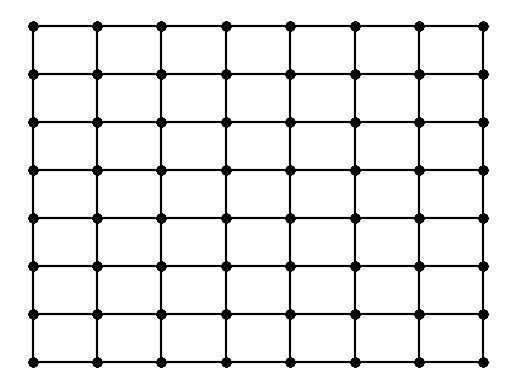
\includegraphics[width=0.3\textwidth]{../figures/structuredGrid}
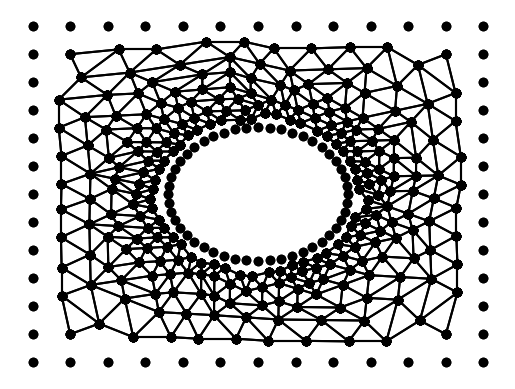
\includegraphics[width=0.3\textwidth]{../figures/unstructuredGrid}
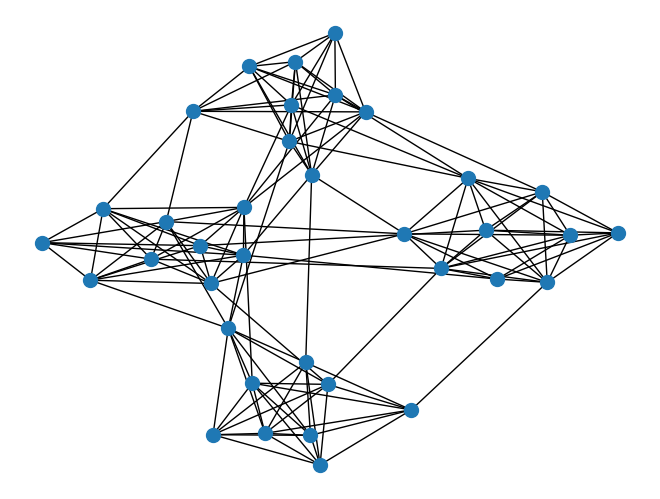
\includegraphics[width=0.3\textwidth]{../figures/graph}
\end{center}
\end{frame}

% Slide
\begin{frame}{Graph problems}
\begin{block}{Lean algebraic multigrid (LAMG)}
\bit
\item Livne and Brandt. Lean algebraic multigrid (LAMG): fast graph Laplacian linear solver. SIAM J. Sci. Comp. 2012.
\item AMG algorithm tailored to solving graph Laplacians for undirected graphs
\item "Lean" because it utilizes simple components designed to optimize cycle efficiency
\bit
\item Gauss-Seidel relaxation
\item Two different coarsening procedures: low-degree elimination and aggregation
\item Piecewise constant interpolation
\item Galerkin coarse-grid operators, $A^c = P^TAP$, are also graph Laplacians 
\eit
\eit
\end{block}
\end{frame}

% Slide
\begin{frame}{Graph problems}
\begin{block}{LAMG coarsening: low-degree elimination}
\bit
\item Low-degree elimination attempts to remove many nodes while adding few edges
\item Removed nodes form an independent set with degree $\leq 4$
\item When a node is eliminated, its neighbors are connected
\item Elimination can be repeated until there are no more (or few) low-degree nodes
\eit
\end{block}
\begin{center}
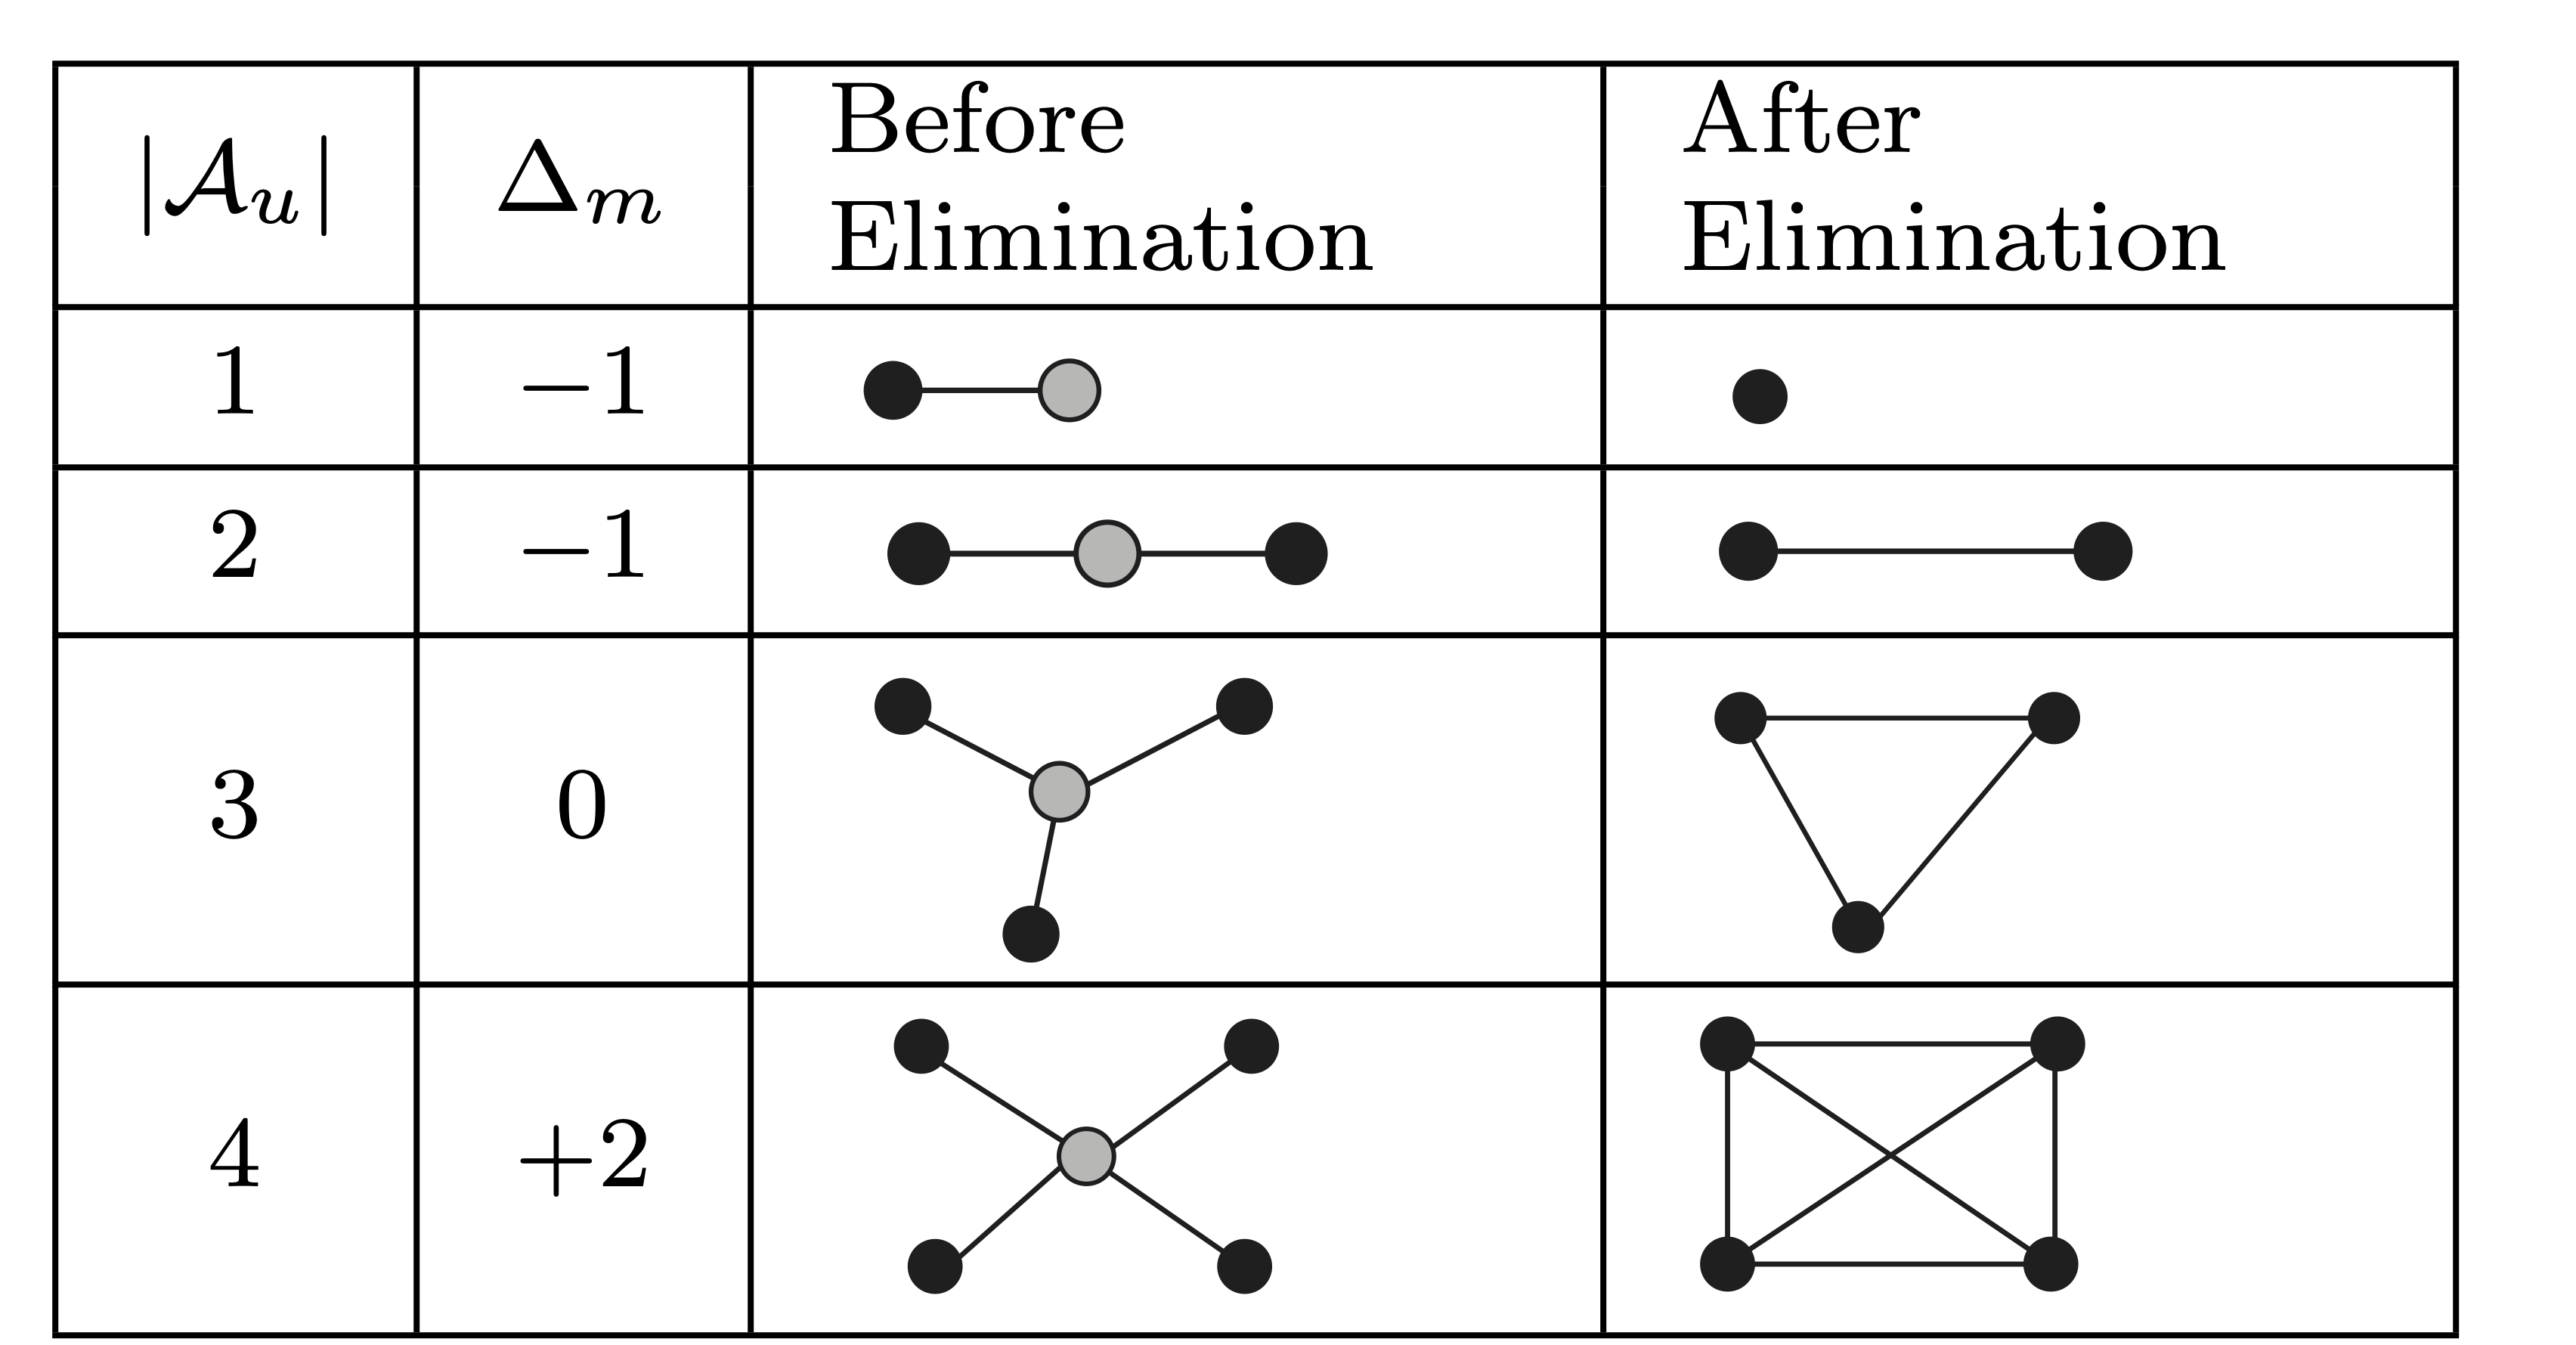
\includegraphics[width=0.4\textwidth]{../figures/lowDegreeElim}
\end{center}
\tiny{Figure credit: Livne and Brandt.}
\end{frame}

% Slide
\begin{frame}{Graph problems}
\begin{block}{LAMG coarsening: aggregation}
\bit
\item Aggregate nodes using "affinity," a modified strength of connection measure based on smoothed test vectors
\item Generate test vectors via a few Gauss-Seidel iterations on $A\mathbf{u} = \mathbf{0}$ with random initial guess
\item Two nodes $i$ and $j$ are highly correlated (and should be aggregated) if $u_i\approx u_j$ for all test vectors, $\mathbf{u}$
\item Approach is similar to adaptive AMG techniques
\eit
\end{block}
\end{frame}

% Slide
\begin{frame}{Graph problems}
\begin{block}{LAMG interpolation}
\bit
\item Interpolation, $P$, is simply piecewise constant interpolation over aggregates
\item This is basically an unsmoothed aggregation AMG approach
\item Sparse $P$ limits fill in for Galerkin coarse-grid operators, $A^c = P^TAP$
\item Reduced interpolation accuracy is overcome through "energy-corrected coarsening" (a modification of the restricted residual)
\eit
\end{block}
\end{frame}

% Slide
\begin{frame}{Graph problems}
\begin{block}{Extensions to LAMG: the signed case}
\bit
\item LAMG was designed for unsigned (all positive edge weights) and undirected (symmetric edges) graphs
\item Signed undirected graphs may have negative edge weights
\item Graph Laplacian has some positive off-diagonals 
\item Diagonal of the graph Laplacian is the total weight, $a_{i,i} = \sum_k |w_{i,k}|$, so $A$ is still diagonally dominant
\eit
\end{block}
\end{frame}

% Slide
\begin{frame}{Graph problems}
\begin{block}{Extensions to LAMG: the signed case}
\bit
\item Fox, Manteuffel, and Sanders. Numerical Methods for Gremban's Expansion of Signed Graphs. SIAM J. Sci. Comp. 2017.
\item Convert a signed graph Laplacian into an unsigned Laplacian and apply LAMG
\item Gremban's expansion: If $S$ is diagonally dominant with positive diagonal, then $S$ may be decomposed as $S = M + P$, where $M$ is a diagonally dominant Z-matrix and $P$ has non-negative entries and zero diagonal. Then the Gremban expansion matrix, $G$, defined by
\eq{
   G = \begin{bmatrix}
   M & -P \\
   -P & M
   \end{bmatrix}
}
is a diagonally dominant Z-matrix.
\eit
\end{block}
\end{frame}

% Slide
\begin{frame}{Graph problems}
\begin{block}{Extensions to LAMG: the signed case}
\bit
\item If $S$ is a signed graph Laplacian, then the resulting $G$ is an unsigned graph Laplacian
\item Solution to $S\mathbf{x} = \mathbf{b}$ can be obtained from the solution to $G\mathbf{w} = \mathbf{z}$
\eq{
   G\mathbf{w} = \begin{bmatrix}
   M & -P \\
   -P & M
   \end{bmatrix}\begin{bmatrix}
   \mathbf{x} \\
   -\mathbf{x}
   \end{bmatrix}
   = \begin{bmatrix}
   \mathbf{b} \\
   -\mathbf{b}
   \end{bmatrix} = \mathbf{z}
}
\item Can also relate the eigenvectors and singular vectors of $S$ and $G$
\item Can apply LAMG successfully to $G$ to solve signed graph problems!
\eit
\end{block}
\end{frame}

% Slide
\begin{frame}{Graph problems}
\begin{block}{Extensions to LAMG: the undirected case}
\bit
\item Fox and Manteuffel. Algebraic multigrid for directed graph Laplacian linear systems (NS-LAMG). Numer. Lin. Alg. Appl. 2018.
\item Undirected graph Laplacians are no longer symmetric
\item Modification of low-degree elimination for the non-symmetric case
\item Modified algorithm to find appropriate test vectors for defining interpolation
\item Coarse grid operators, $A_c = RAP$, where $R\neq P^T$
\eit
\end{block}
\end{frame}

%%%%%%%%%%%%%%%%%%%%%%%%%%%%%%%%%%%%%%%%%%%%%%%%%%%%%%%%%%%%%%%%%%%%%%%%%%%%%%%%

\end{document}

